\chapter{Theory and Methods}
\label{chap:theory}

In this chapter the theoretical background and the methods used in this work are presented. This includes the collection of research on the fungal species Cladosporium sphaerospermum, as well as the atmospheric pressure plasma and the different processes that lead to the sterilization of the mould as they interact. 

\section{Cladosporium sphaerospermum}
Cladosporium sphaerospermum (C. sphaerospermum) is a species of fungus. Fungi are a large group of eukaryotic organisms\footnote{Organisms whose cells have a membrane around their nucleus, which includes animals, plants and fungi.}  that include yeasts, moulds and common mushrooms. It is a black mould that is commonly found in indoor environments, especially in areas that are damp or have high humidity. It was first described by a German mycologist, Albert Julius Otto Penzig, in 1886 from decaying citrus plant material in Italy \cite{mould}. C. sphaerospermum primarily reproduces asexually through the production of conidia, which are non-motile spores\footnote{Spores not capable of movement.} formed at the tips of hyphae\footnote{Long, branching structures that grow from their tips. They give moulds their furry appearance.}. These spores are easily dispersed through the air, allowing the mould to rapidly spread into new environments. Moulds like C. sphaerospermum require humid conditions because moisture is essential for spore germination\footnote{The process by which a spore begins to grow new hyphae.}. In dry environments, spores usually remain dormant \cite{growth}.

\subsection{Growth and Morphology\footnote{The study of the structure of organisms.}}
C. sphaerospermum has a darkly-pigmented mycelium\footnote{A network of branching hyphae.} that can appear black or dark green. The colonies of the mould are typically flat and have more of a powdery appearance than other moulds. It is typical for fungi of the Cladosporium family to have branching, tree-like hyphae on whose ends conidia are formed in chains. The spores themselves are round to oval in shape and measure a few micrometers in length. They are very resilient and can stay alive even in conditions not favourable for growth. Due to their small size they are invisible to the naked eye. In Figure \ref{fig:mould} the morphology of C. sphaerospermum is shown. 

In addition to a humid environment optimal conditions for the growth of C. sphaerospermum include a temperature of 25  \textdegree C. It is however a  psychrophilic fungus\footnote{An organism that is able to grow in very low temperatures.} and can grow at temperatures as low as -5 \textdegree C \cite{mould}. It nourishes through saprotrophic nutrition, which is the process of using decaying or dead organic matter as a source of nutrients. This is why it is commonly found in decaying plant material, where it was also discovered. The conversion of starch, cellulose and other compounds such as carbon dioxide provides the energy needed for growth.

\begin{figure}
    \centering
    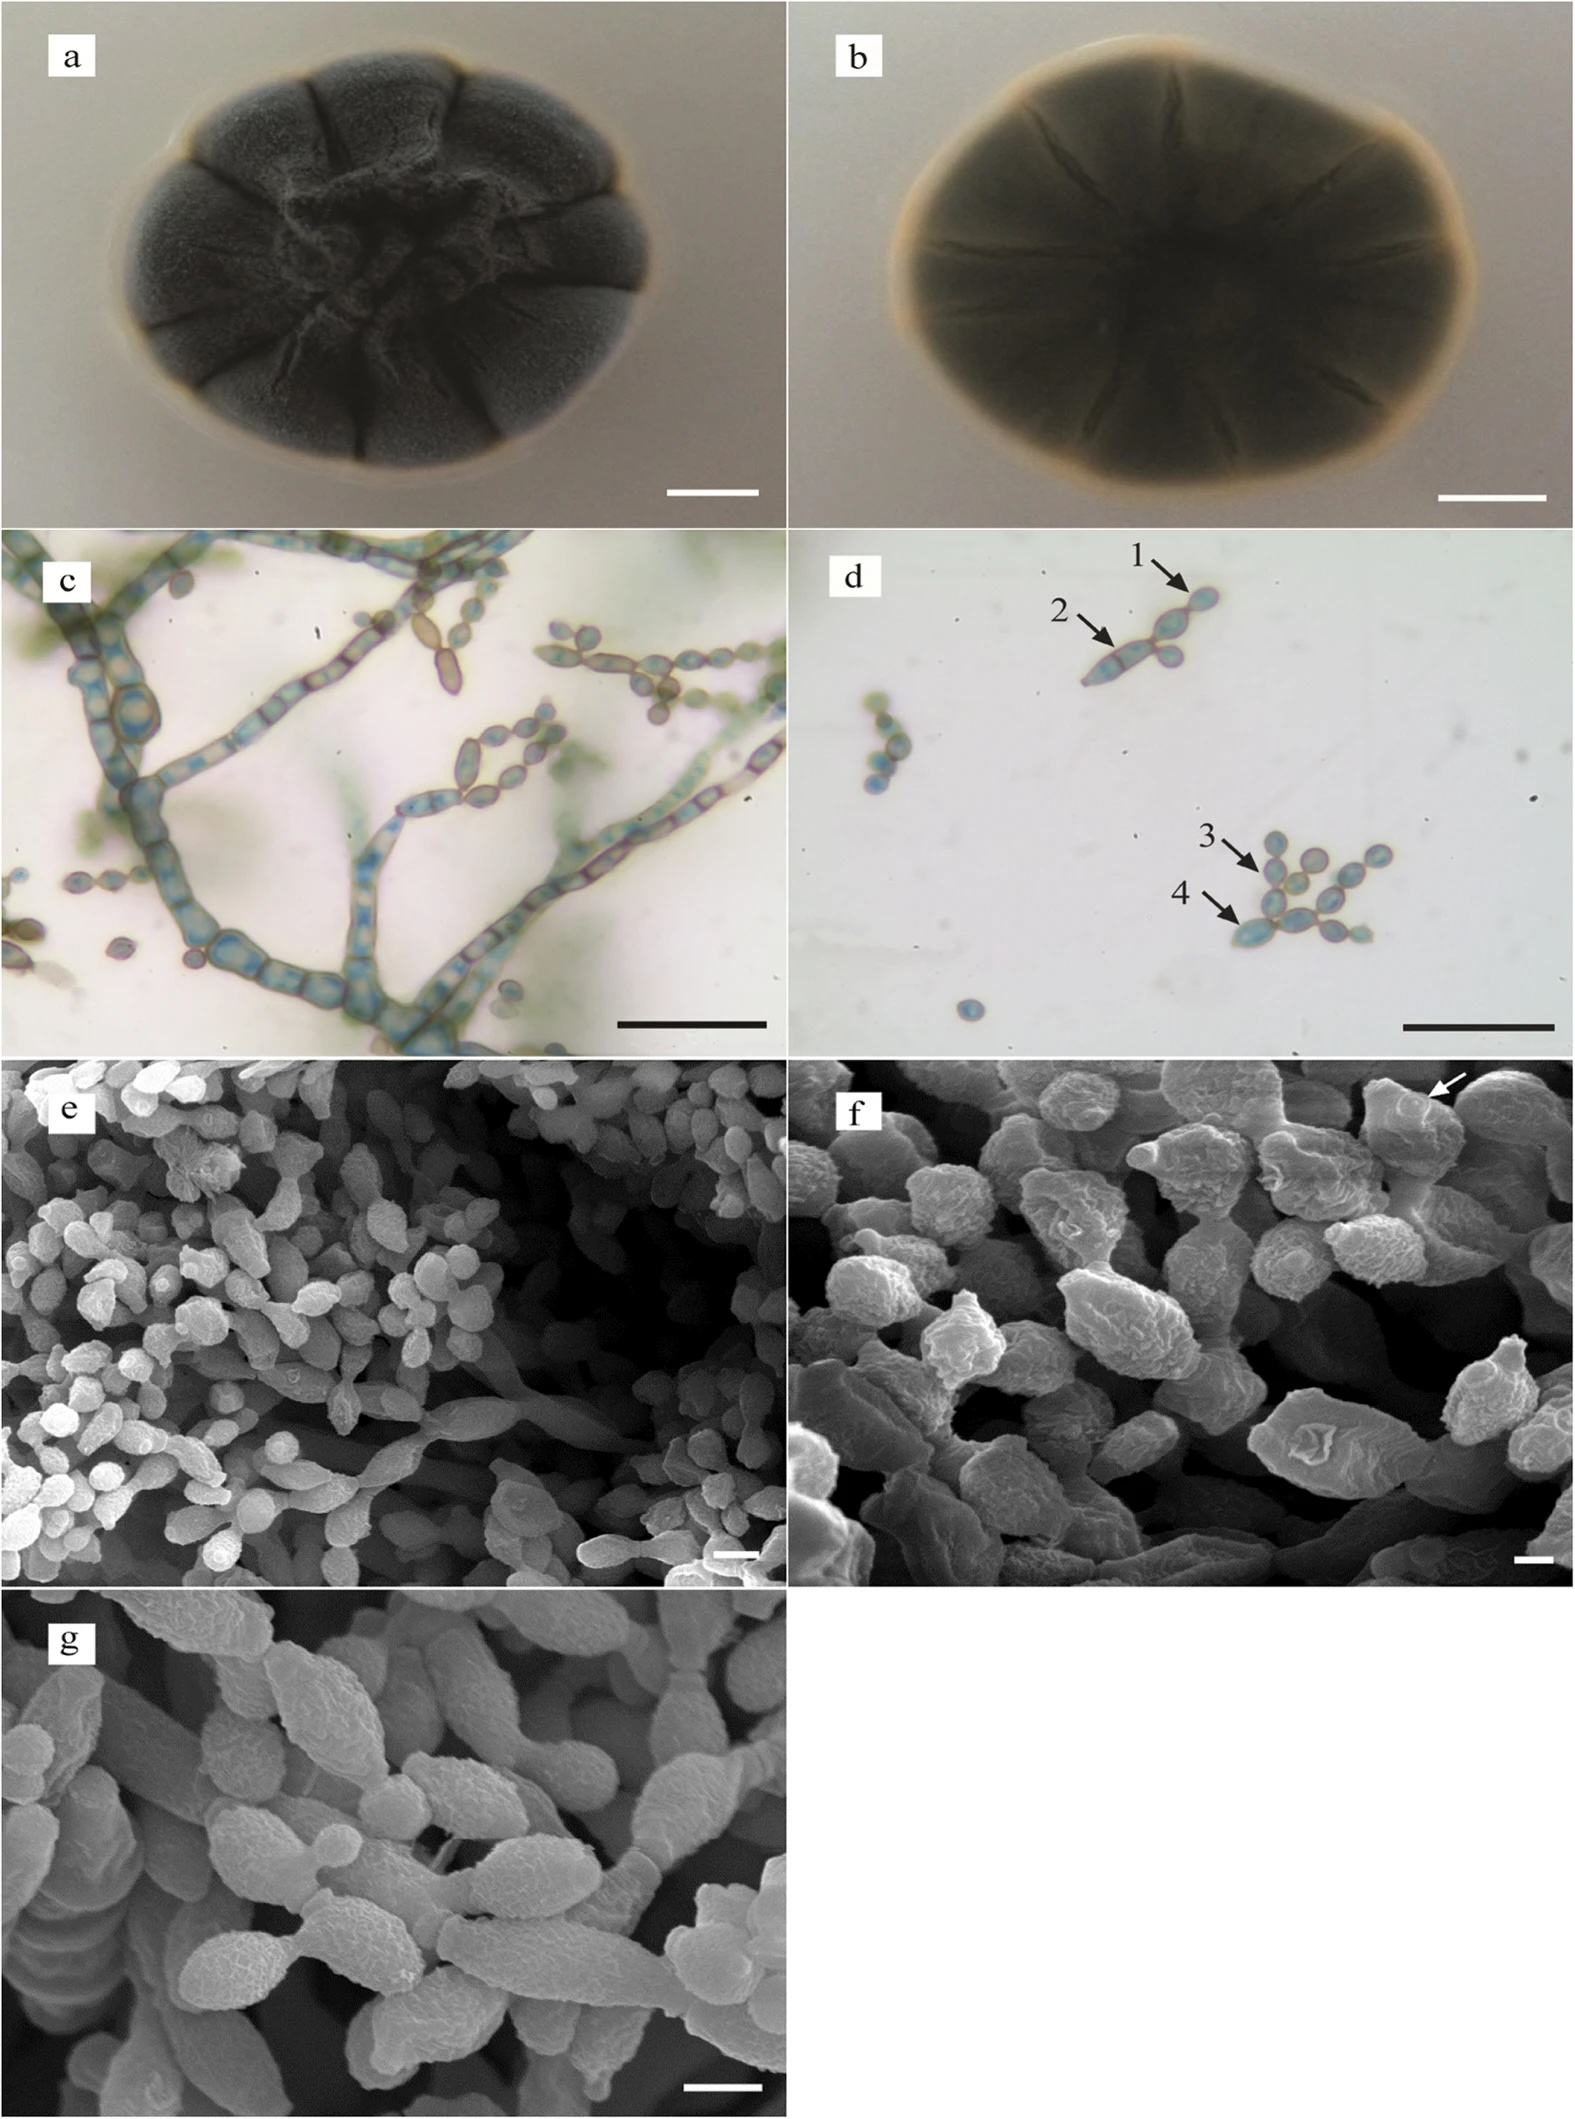
\includegraphics[width=.85\textwidth]{images/mould.jpg}
    \caption[Morphology of C. sphaerospermum]{Morphology of C. sphaerospermum from \cite{morphology}. Colonial morphology front (a) and reverse (b) of C. sphaerospermum UM 843 on SDA after 7-day incubation. Light micrograph showing conidia (d 2 and d 4). $\times$630 magnification, bars 20 \textmu m. Observation under scanning electron micrograph showing (e,f,g) conidiophores bearing conidium (e, $\times$2000 magnification, bar 3 \textmu m), periclinal rim\footnotemark. (f, $\times$5000 magnification bar 1 \textmu m) and verruculose surface of conidia (g, $\times$5000 magnification, bar 2 \textmu m).}
    \label{fig:mould}
\end{figure}

\subsection{Ecological Role and Occurrence}
Like many fungi C. sphaerospermum plays an important role in the ecosystem as a decomposer. It breaks down dead organic matter, recycling nutrients back into the soil, where it thrives. This process is important as it fertilizes the soil and allows for the growth of new plants, enabling the life cycle. Because of its resilience to different conditions it is able to grow in many different environments which include anthropogenic places like indoor environments. In humid areas and on porous surfaces, such as wood or concrete walls it can build mycelium and produce new spores. The easily dispersed spores reach virtually everywhere and are even found in orbiting spacecraft \cite{radiation}.

While fungi don't perform photosynthesis and therefore do not convert CO$_2$ into oxygen they still contribute to the carbon cycle. By digesting plant material and binding carbon dioxide in their biomass they play an important role in storing carbon and reducing the amount of carbon dioxide released into the atmosphere when plants decay. Because of there abundance they are able to store large amounts and help build stable compounds for long-term soil carbon storage.

\footnotetext{The outer edge of a cell wall layer formed parallel to the spore surface.}

\subsection{Effects on Human Health}
Because of its ubiquity C. sphaerospermum surrounds humans in their daily lives. The small size of the spores allows them to be inhaled deeply into the lungs where they can lead to allergenic reactions as well as pathogenic infections\footnote{A pathogen is any organism that can cause disease in a host.}, particularly when the immune system is weakened. Compared to other airborne moulds it is however not considered a serious health risk as it does not produce mycotoxins\footnote{Toxins produced by certain fungi that can cause severe disease in humans and animals.}. Fungi in general can cause respiratory problems, especially when inhaling them in large quantities over a long time. They are however also essential in medical science as they are used to produce antibiotics, such as penicillin. While working with them in the lab clean benches can be used to provide sufficient ventilation but they generally don't pose any danger to a healthy person.

\subsection{Response to Radiation}
\label{sec:radiation}
UV radiation is commonly used to sterilize surfaces and is very effective in killing most microorganisms like bacteria and fungi. C. sphaerospermum however shows a higher resistance to different types of radiation including UV and even high energy ionizing radiation.  
It is able to not only survive doses of ionizing radiation that would kill most other organisms but also to thrive in these conditions. This was discovered in 1990s as the fungus is able to grow in the high radiation environment of the destroyed Chernobyl nuclear power plant \cite{radiation}, even on the highly radioactive reactor walls. The mould does not only survive in these conditions but was proposed to be radiotrophic - a process where fungi potentially use ionizing radiation as a source of energy analogous to photosynthesis - growing faster.

Its tolerance to radiation both ionizing and non-ionizing is attributed to the pigment molecule Melanin. Pigment molecules such as Melanin absorb visible light and other radiation which can protect cells, can be used to absorb energy. It gives the mould its dark colour and protects its from UV radiation. Melanin is also able to absorb ionizing radiation and potentially convert it into chemical energy usable to the fungus.

To further research this discovery the mould was sent to the International Space Station in 2018 where it was exposed to cosmic radiation \cite{iss}. The study found that the mould was able to survive the radiation and even thrive in the microgravity environment while absorbing some of the energy. The results of the study suggest that C. sphaerospermum could potentially serve as a highly sought-after solution for creating a self-replicating biological radiation shield or be otherwise useful in space exploration.

\section{Atmospheric Pressure Plasma}
A plasma is a state of matter that consists of ionized gas and free electrons. The particles behave collectively in a highly dynamic way because they are coupled closely through electromagnetic fields. The state is also conductive and the plasma can be influenced by external electric and magnetic fields \cite{plasma}. Although the particles carry charges locally, a plasma is electrically neutral when observed as a whole. Plasmas can be created by applying energy in the form of heat or electromagnetic fields to a gas. To ignite a plasma at low temperatures, a discharge is needed, the conditions for which - such as pressure, voltage and distance - are described by Paschen's law. This law states that it is generally easier to create a plasma in a low-pressure environment, as the mean free path (the distance between particle collisions) is larger, allowing the electrons to gain more energy before colliding with other particles, so they can exceed the ionization threshold. This is why many plasmas are created in vacuum chambers. However, with a sufficiently high voltage, it is  possible to create plasma at atmospheric pressure also. Such a plasma is known as an atmospheric pressure plasma (APP). APPs have the advantage of being comparatively simple to handle as no vacuum vessel is required to contain them. This also makes it easier to bring them into the proximity of samples for various applications such as sterilization, surface treatment or material processing \cite{plasma}. To sustain the plasma an alternating current in the Kilohertz range is used, so that the changing electromagnetic field is able to accelerate electrons continuously. The much heavier ions are accelerated only minimally in comparison. Although electron temperatures commonly reach around 10$^4$ K, it is possible to sustain a plasma at room temperatures if the energy provided is controlled \cite{plasma2}. Such plasmas are referred to as cold plasmas or non-thermal plasmas. Because of the high voltage required to ignite APPs arc discharges can occur between the electrodes which significantly reduce the plasma stability. This makes it very hard to predict their behaviour and would heat them up to much higher gas temperatures which needs to be prevented for many experiments. Dielectric barriers can be used to achieve a controlled discharge and energy transfer. 

Many processes occur in a plasma besides ionization. The gas atoms are also frequently excited which leads to the emission of photons as these states are non-stable which gives plasmas their characteristic glow. Molecules can also be dissociated by collisions which leads to the formation of radicals and other chemical bonds that can have varying lifespans. The radiation as well as the reactive species produced in the plasma allow the plasma to interact with surfaces and materials in its proximity.

\section{Dielectric Barrier Discharge}
To achieve a controlled non-thermal plasma at atmospheric pressure a dielectric barrier discharge (DBD) can be used. This means that the two electrodes that carry the high voltage to ignite and sustain the plasma are separated by a dielectric barrier. There are different configurations to realize this. Some setups use only one dielectric barrier at one of the electrodes while commonly both electrons - planar or cylindrical - are covered with a dielectric material. The dielectric barrier is a non-conductive material that prevents the formation of an arc discharge between the electrodes but can be polarized by the electric field. Often glass, quartz or ceramics are used for this purpose. While the plasma is ignited the dielectric barrier prevents the electrons from flowing freely between the electrodes and charges are built up on the surface of the dielectric. This stops the discharge very quickly and thereby limits the current flow, an alternating current is needed. By controlling the voltage and frequency of this current the discharge can be sustained in a stable way. The dielectric barrier also helps to create a uniform electric field similar to its use in capacitors. 

DBD is used widely in different applications that require a non-thermal plasma like the semiconductor or medical industry. It is used for surface treatment, cleaning and sterilization, like in this work, where a cold plasma is needed that does not destroy the surfaces it interacts with. It is interesting

\section{Optical Emission Spectroscopy}
Optical emission spectroscopy (OES) uses the electromagnetic radiation emitted by a plasma to analyse its composition. This can be done non-intrusively meaning that the plasma does not need to be disturbed and remains unaffected by the measurement. That is a major advantage when working with small volumes of plasma like in this work where probes would significantly change the conditions \cite{plasma2}. OES measures a spectrum of the emitted light which gives the intensity at different wavelengths. Because the photons originate from distinct transitions between energy levels sharp peaks are observed in the spectrum. Their wavelength can be used to identify the species that are present in the plasma as well as the processes that occur. This also allows an estimate of the plasma temperature and the concentration of the different gases in the plasma, although more information like cross-sections for the different processes is needed \cite{plasma2}. Boltzmann plots are often used to derive the electron temperature from the measured spectrum, however they assume local thermal equilibrium which is not the case in non-thermal plasmas. This means that the electron temperature is not equal to the gas temperature and the Boltzmann plot can only be used as an approximation \cite{plasma2}. 

In OES one needs to account for the spectrometer's spectral response, which is the sensitivity of the detector per wavelength. This is usually done by measuring a calibration spectrum and correcting the measured spectrum accordingly. 

\section{Sterilization Mechanism}
APPs have been used for sterilization of surfaces in many studies as outlined in chapter \ref{chap:scientific_context}. Although the plasma is not in direct contact with the sample two main mechanism have been found to be responsible for the sterilization effect. The first is the radiation emitted by the plasma, which can be UV or visible light. The second is the reactive species that are produced in the plasma and interact with the surface. Additionally, heat as well as electric fields can also play a role in the sterilization process. The exact mechanism is still subject to research and what process dominates depends on the specific setup and sample. This study aims to test and isolate the effects of the radiation and reactive species on the inactivation of C. sphaerospermum. The following sections will discuss what is known about the different processes and how contribute to the sterilization.

\subsection{Reactive Species}
As discussed in chapter \ref{chap:scientific_context} the main mechanism for the inactivation of microorganisms in prior studies appeared to be the reactive species produced in the plasma. Because of the high electron temperatures in the plasma some electrons gain enough energy to dissociate molecules and create radicals. When working with an APP the main gases present are oxygen and nitrogen as well as water vapour. The most important reactive species produced are hydroxyl radicals (OH) and ozone (O$_3$). Radicals are missing an electron and are therefore highly reactive chemicals. They are widely used in water treatment and sterilization because they can react with organic compounds and degrade them \cite{water}. Studies such as \cite{ozone} have demonstrated that the concentration of ozone can be correlated with the rate of microbial inactivation directly. These reactive species can penetrate cells and cause damage to vital biomolecules, including DNA and proteins.
This leads to the inactivation of the microorganism as it is unable to reproduce or perform its normal functions and was proven to be effective against the spores of C. sphaerospermum \cite{kit}. By using chemical probing methods the concentration of reactive species can be measured. For example the concentration of OH radicals can be quantified by their fluorescence when they are reacted with a chemical probe such as sodium terephthalate (NaTA). 

\subsection{Radiation Effects}
In addition to the radicals produced by the plasma it emits radiation that interacts with the sample. In APP visible light as well as UV light in the UV-A and UV-B range is typically emitted \cite{plasma2}. UV radiation is used a lot for sterilization and is standard in many clean benches used in laboratories but slightly higher frequencies in the UV-C range are used. A study by Li, Yiqian and others \cite{bacteria} found that plasma emitting UV-A and UV-B light can have a significant effect on the inactivation rate of bacteria when using a quartz-glass separation but that the shorter wavelengths are more effective.

The main reason why UV radiation is effective at killing microorganisms is its photochemical interaction with DNA. DNA is very susceptible to absorption of UV light which can alter its structure leading to the breaking of bonds and the formation of mutations \cite{DNA}. DNA contains four bases: adenine (A), thymine (T), cytosine (C), and guanine (G). These are all aromatic molecules. Aromatic molecules are ring-shaped compounds with delocalized \text{$\pi$-electrons}, meaning their electrons are not confined to individual bonds but can move freely within the molecule \cite{DNA}. This makes them highly stable, but the electrons can efficiently  be excited by  UV light, especially around 260 nm. The transition \begin{equation}
    \pi \rightarrow \pi ^\star,
\end{equation}
describes the excitation of an electron from a bonding\footnote{A bonding orbital results from constructive interference of atomic orbitals, lowering electronic energy.} $\pi$-orbital to an anti-bonding\footnote{An anti-bonding orbital results from destructive interference of atomic orbitals, raising electronic energy.}  $\pi^\star$-orbital. This significantly weakens the bonds in the molecule and can lead to the formation of dimers\footnote{In DNA, dimers can form when two adjacent bases bond abnormally due to UV exposure \cite{DNA}.}. Fungi just like bacteria rely on the integrity of their DNA as it is the basis for their reproduction of cells, which makes any damage to the DNA highly effective in killing them.

As mentioned in section \ref{sec:radiation} C. sphaerospermum is more resistant to UV radiation than bacteria because it is a melanized fungus. Melanin helps to protect the DNA from UV radiation by absorbing some photons before they reach the DNA. This means higher doses are necessary to achieve the same inactivation rate.